% 2019-04-03

\documentclass[10pt]{article}
\usepackage[T1]{fontenc}
\usepackage{amssymb}
\usepackage{amsmath}
\usepackage{graphicx}
% \begin{figure}[h]
% \centering
% \includegraphics[width=6.5in]{folder/photo.png}
% \caption{}
% \label{}
% \end{figure}



\usepackage{tikz}
\usetikzlibrary{arrows}
\usepackage{subfigure}
\usepackage{stackrel}
\usepackage{blindtext}

\usepackage{biblatex}
\addbibresource{library.bib}

\oddsidemargin=0.15in
\evensidemargin=0.15in
\topmargin=-.5in
\textheight=9in
\textwidth=6.25in

\usepackage[colorlinks=true,breaklinks,pdfpagemode=none,linkcolor=blue,citecolor=blue]{hyperref}

\usepackage{enumerate}
% \vspace{-6pt}
% \begin{itemize}
%     \setlength{\itemsep}{0pt}%
%     \setlength{\parskip}{0pt}%
%     \item Item 1
%     \item Item 2
%         \begin{itemize}
%             \setlength{\itemsep}{0pt}%
%             \setlength{\parskip}{0pt}%
%             \item Sublist Item 1
%             \item Sublist Item 2
%         \end{itemize}
%         \item Item 3
% \end{itemize}
% \vspace{-6pt}


\usepackage{enumitem}
\setlist{itemsep=0mm}

\usepackage{scrextend}

\usepackage{amsmath,amsfonts,amssymb,bm}


\begin{document}

   \noindent
   \begin{center}

   \hrulefill
   
   \vspace{5pt}
   
   \makebox[\textwidth]{ {\bf Energy Systems Analysis} \hfill  A.D. Smith 2019}
   \vspace{0pt}
   
   {\Large \hfill  Lecture 29.  
Demand Side Energy Management Strategies
}
   \vspace{5pt}
   
  
   \hrulefill
   \end{center}
   
    {\color{darkgray}{\center{ \small{      ``[Demand response] is a great cousin of energy efficiency, but it is not a substitute for the fundamental process of replacing inefficient energy-using capital, or building in more efficiency in the first place.''
\\%[3pt]
\rightline{{\rm --- Peter Fox Penner \cite{Fox-Penner2014-nv}}}}}}}


\section{What are demand side energy management strategies?}

We can broadly classify distributed energy resources into:

\begin{itemize}
    \item Power generation
    \item Energy storage
    \item Energy management
\end{itemize}

Distributed power generation happens at the site, and distributed storage provides an option to help alleviate a mismatch between supply and demand. Energy management captures the options we have on the \textit{demand side} of the electrical grid to reduce energy use, often in very targeted ways, such as reducing power use during peak times for the grid. 

You may recall that OpenStudio breaks energy systems into supply and demand sides within an individual building or facility based on supply (e.g. chiller) and demand (e.g. VAV box) equipment, as illustrated in Figure \ref{os-s-d}. Here, we're now speaking from a larger perspective so that supply comes from central facilities (left side of Figure \ref{u-s-d}) or from distributed power generation (middle of Figure \ref{u-s-d}), and demand is the whole building's energy requirements (right side of Figure \ref{u-s-d}). If you're a grid operator, buildings have traditionally been your demand and power was supplied to non-industrial facilities from grid-level power plants. That is changing---buildings and distributed generation are becoming more significant producers of electrical energy, and what we view as 'supply' is changing as well---we  now have \textit{virtual power plants (VPP)} participating in electricity markets \cite{Cohn2018-ja}.

            \begin{figure}[h]
            \centering
            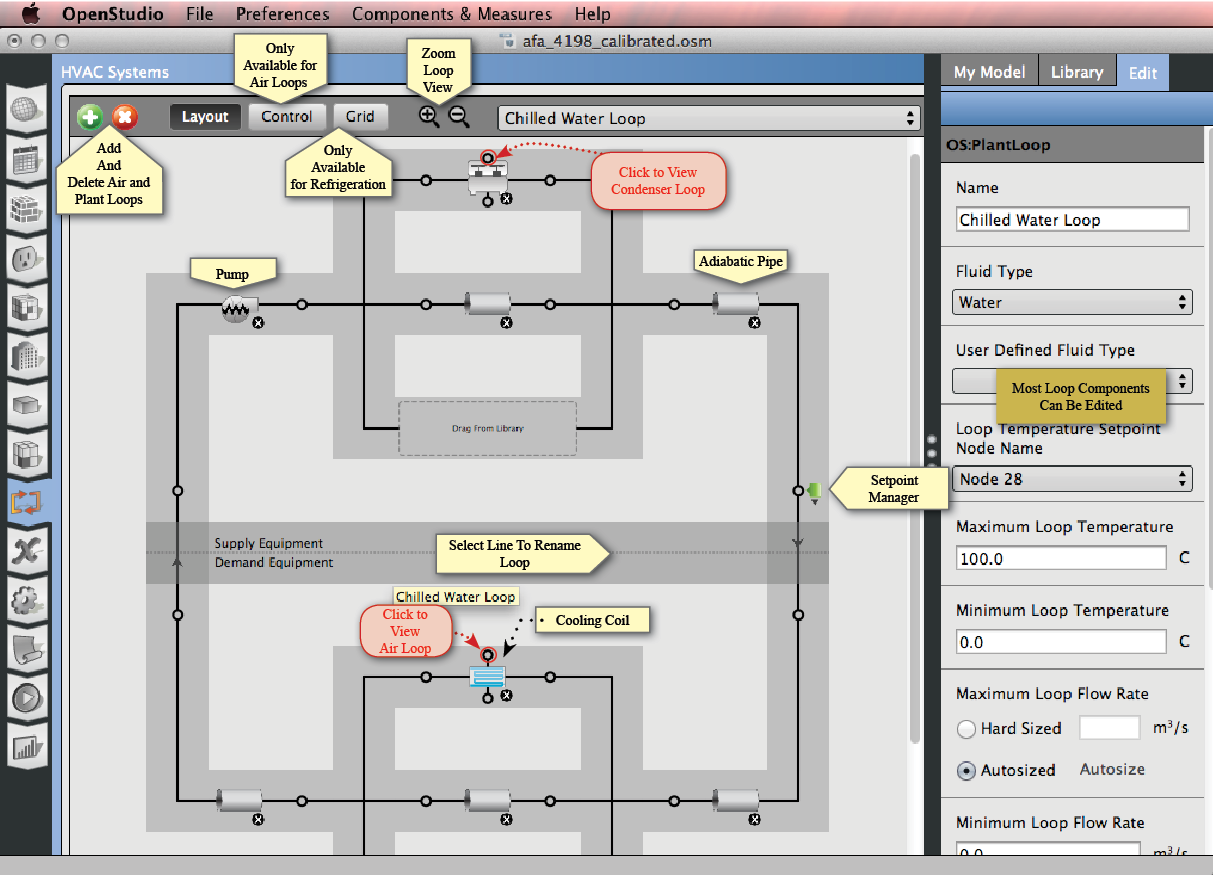
\includegraphics[width=13cm]{extras29/OS-supply-demand.png}
            \caption{Chilled water system model as shown in the OpenStudio interface \cite{OSdocs}}
            \label{os-s-d}
            \end{figure}
            
                        \begin{figure}[h]
            \centering
            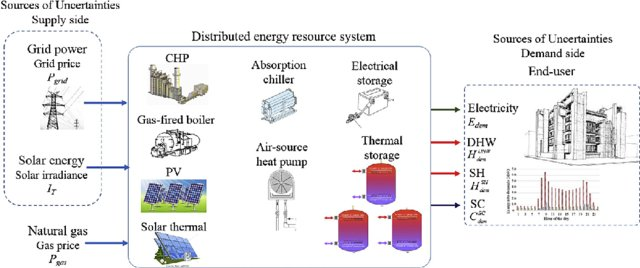
\includegraphics[width=15cm]{extras29/uncertainty-supply-demand.jpg}
            \caption{Representative scheme of a distributed energy resource system illustrating sources of uncertainties of supply and demand sides  \cite{Di_Somma2018-fa}}
            \label{u-s-d}
            \end{figure}




\section{Energy management terminology}

These are some of the key terms we'll run into when considering demand-side energy management options, from both a building-level and a grid-level perspective. You may see these used in slightly different ways in other places, but we will stick with the definitions used by the U.S. Energy Information Administration (EIA).

\begin{labeling}{Global sensitivity analysisx}

\item [\textbf{Conservation}] ``reduction in energy consumption that corresponds with a reduction in service demand. Service demand can include buildings-sector end uses such as lighting, refrigeration, and heating; industrial processes; or vehicle transportation. Unlike energy efficiency, which is typically a technological measure, conservation is better associated with behavior.''  \cite{EIAglossary}

\item [\textbf{Demand charge}]  ``portion of the consumer's bill for electric service based on the consumer's maximum electric capacity usage and calculated based on the billing demand charges under the applicable rate schedule.''  \cite{EIAglossary}

\item [\textbf{Demand interval}]  ``time period during which flow of electricity is measured (usually in 15-, 30-, or 60-minute increments.)''  \cite{EIAglossary}


\item [\textbf{Demand response programs}] ``incentive-based programs that encourage electric power customers to temporarily reduce their demand for power at certain times in exchange for a reduction in their electricity bills. Some demand response programs allow electric power system operators to directly reduce load, while in others, customers retain control\ldots'' \cite{EIAglossary} The infographic in Figure \ref{a-d-r} explains the basics of a demand response program in general. The Australian Renewable Energy Agency has published a nice high-level explanation online called ``The power of a simple idea: What is demand response?'' \cite{Arena_undated-cl}.

\item [\textbf{Demand-side management}] ``A utility action that reduces or curtails end-use equipment or processes. DSM is often used in order to reduce customer load during peak demand and/or in times of supply constraint\ldots''

\item [\textbf{Energy efficiency}]  ``ratio of service provided to energy input (e.g., lumens to watts in the case of light bulbs). Services provided can include buildings-sector end uses such as lighting, refrigeration, and heating: industrial processes; or vehicle transportation. Unlike conservation, which involves some reduction of service, energy efficiency provides energy reductions without sacrifice of service.'' \cite{EIAglossary}

\item [\textbf{Energy management practices}]  ``Involvement, as a part of the building's normal operations, in energy efficiency programs that are designed to reduce the energy used by specific end-use systems.''  \cite{EIAglossary}

\item [\textbf{Load control program}] ``program in which the utility company offers a lower rate in return for having permission to turn off the air conditioner or water heater for short periods of time by remote control. This control allows the utility to reduce peak demand.'' \cite{EIAglossary}

\item [\textbf{Load leveling}] ``load control technique that dampens the cyclical daily load flows and increases baseload generation. Peak load pricing and time-of-day charges are two techniques that electric utilities use to reduce peak load and to maximize efficient generation of electricity.'' \cite{EIAglossary}

\item [\textbf{Load shedding}] ``intentional action by a utility that results in the reduction of more than 100 megawatts (MW) of firm customer load for reasons of maintaining the continuity of service of the reporting entity's bulk electric power supply system\ldots'' \cite{EIAglossary}

\item [\textbf{Peak load}]  ``maximum load during a specified period of time.''  \cite{EIAglossary}

\item [\textbf{Off peak}]  ``Period of relatively low system demand. These periods often occur in daily, weekly, and seasonal patterns; these off-peak periods differ for each individual electric utility.''  \cite{EIAglossary}

\item [\textbf{Rate schedule (electric)}] ``rates, charges, and provisions under which service is supplied to the designated class of customers.'' \cite{EIAglossary}

\item [\textbf{Time-of-day rate}]  ``rate charged by an electric utility for service to various classes of customers. The rate reflects the different costs of providing the service at different times of the day.''  \cite{EIAglossary}

\end{labeling}

            
                        \begin{figure}[h]
            \centering
            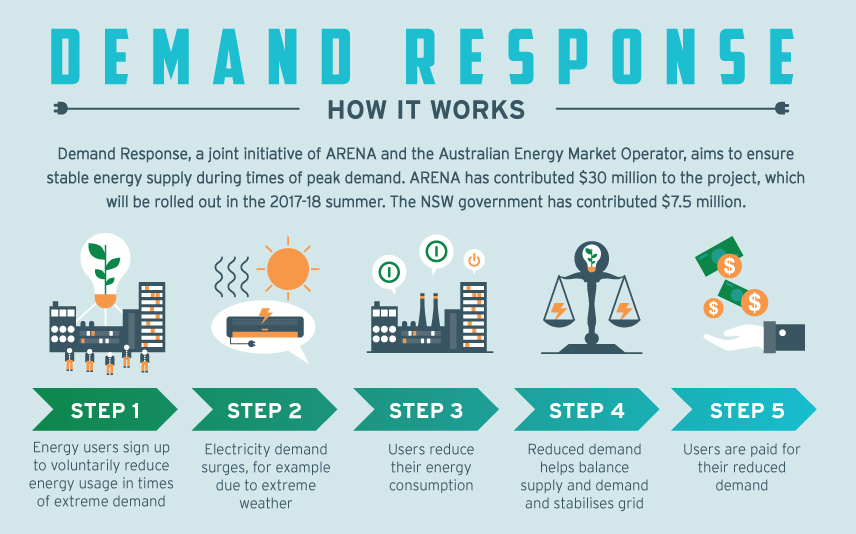
\includegraphics[width=16cm]{extras29/demand-response.jpg}
            \caption{Basic idea behind demand response as illustrated by the Australian Renewable Energy Agency \cite{Arena_undated-cl}}
            \label{a-d-r}
            \end{figure}



You may also run into alternate phrasings and related terms like ``real-time pricing,'' implying pricing that varies in small time intervals (hourly or sub-hourly) and from day to day, similar a time-of-day rate, which will likely be grouped into time blocks and will be more consistent over time, and ``dynamic pricing'' which is usually used as a synonym for real-time pricing.




% FLATTENING the duck
% https://www.nrel.gov/news/program/2018/10-years-duck-curve.html

% license
\bigskip

\noindent
\texttt{\footnotesize RESTRICTED PUBLIC LICENSE --- READ BEFORE SHARING. This is a draft version made available by Amanda D. Smith under a Creative Commons Attribution-NonCommercial-ShareAlike license. 
\href{https://creativecommons.org/licenses/by-nc-sa/4.0/}{CC BY-NC-SA 4.0}}

\medskip

% references
\newpage
\printbibliography

\end{document}